\documentclass{lecturenotes}

\renewcommand{\vecka}{13}
\newcommand{\tema}{Designexempel}

\setbeamertemplate{footline}[frame number]
\title[Föreläsningsanteckningar EDA016, 2015]{EDA016 Programmeringsteknik för D}
\subtitle{Läsvecka \vecka: \tema}
\author{Björn Regnell}
\institute{Datavetenskap, LTH}
\date{Lp1-2, HT 2015}

%%%%%%%%%%%%%%%%%%%%%%%%%%%%%%%%%%%%%%

\begin{document}

\frame{\titlepage}
\setnextsection{\vecka}
\section[Vecka \vecka: \tema]{\tema}
\frame{\tableofcontents}

\subsection{Att göra denna vecka}
\begin{Slide}{Att göra i Vecka \vecka: Studera designexempel.}
\begin{enumerate}
\item Läs följande kapitel i kursboken:  10.4, 10.5, 12.7 \\  
  Designexempel: Myntvändning, Nim-spel, Hanois torn
\item Gör extraövningar (inkl. kolla på lösningsförslag) \\ {\scriptsize \url{http://fileadmin.cs.lth.se/cs/Education/EDA016/exercises/extraexercises.pdf}}
\item Träffas i samarbetsgrupper och hjälp varandra 
\item Diskutera \Emph{inlämningsuppgiftsval} med handledare 
\item Gör Grupplabb 11: Image Filters
\end{enumerate}
\end{Slide}

\subsection{Riktlinjer inlämningsuppgift}
\begin{Slide}{Riktlinjer inlämningsuppgift}
Mål: Visa att du kan ska skapa ett större program. 
\begin{enumerate}

\item Välj bland 3 alternativ eller hitta på en egen som uppfyller: 
\begin{enumerate}
\item Minst ca 500 rader, minst 5 klasser, gärna mer.
\item Skapa egna klasser som samverkar.
\item Använda färdiga klasser.
\item Använda en datastruktur, till exempel ArrayList.
\item Avlusa och förbättra ditt program stegvis.
\end{enumerate}

\item Diskutera val av uppgift med handledare denna vecka.

\item Förbered presentation till redovisningen.
\end{enumerate}
Läs mer i kompendiet på sid 89.
\end{Slide}

\subsection{Repetition: Vad är en algoritm?}
\begin{Slide}{Repetition: Vad är en algoritm? }\footnotesize
En \href{https://sv.wikipedia.org/wiki/Algoritm}{algoritm} är en stegvis beskrivning av hur man löser ett problem. \\ 
\vspace{1em}
Problemlösningsprocessens olika steg (inte nödvändigtvis i denna ordning): 
\begin{enumerate}
\item identifiera (del)\Emph{problemet}
\item Kom på en \Emph{lösningsidé}
\item Formulera en \Emph{stegvis beskrivning} som löser problemet
\item Implementera en \Emph{körbar lösning} i ''riktig'' kod
\end{enumerate}
Det krävs ofta \Emph{kreativitiet} i alla steg ovan  -- även i att \Emph{känna igen} problemet.
\end{Slide}

\subsection{Design av mjukvara}
\begin{Slide}{Delar i designprocessen för utveckling av mjukvara}
\begin{itemize}
\item Krav: Varför? Vad? \\ Intressenter, önskelmål, produktstartegier, beslut
\item Arkitektur: struktur och principiell design
\item Design: Hur? \\ Uppdelning i delproblem, vilka klasser? vilka API?
\item Implementation: Hur? \\ 
Algoritmer, kod, implementera API
\item Testning: Är det rätt kvalitet? \\ Enhetstest, Modultest, Systemtest, Acceptanstest
\item Hantera byggprocessen och olika versioner
\item Driftsättning \Eng{Deployment} 
\item Drift \Eng{Operation}
\item Support och återkoppling
\end{itemize}
\end{Slide}

\begin{Slide}{Designexempel i ankboken}
\begin{itemize}
\item Kap. 10.4: Myntvändning  -- Läs själv!
\item Kap. 10.5: Nim-spel -- Läs själv!
\item Kap. 12.7:   \Emph{Hanois torn}
\item (Kap. 16.6:  Swing-program; mer om GUI i fk med JavaFX)
\end{itemize}
\end{Slide}

\Subsection{Towers of Hanoi}
\begin{Slide}{Designexempel: Hanois torn}
Det finns tre pinnar numrerade 1, 2, 3. Från början finns $n$ brickor av avtagande storlek på pinne 1 med den största brickan underst. Pinne 2 och pinne 3 är tomma.
\begin{center}
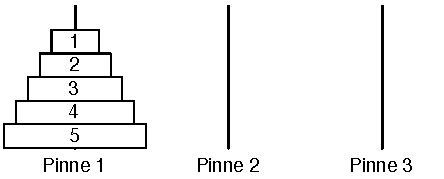
\includegraphics[scale=0.9]{img/hanoi-init.pdf}
\end{center}
De $n$ brickorna ska flyttas så att de hamnar i \Emph{avtagande} storlek på en av de övriga pinnarna. Detta ska ske i en följd av drag där man i varje drag flyttar den \Emph{översta} brickan från en pinne till en annan pinne. \Emph{Den bricka som flyttas får \Alert{aldrig} placeras ovanpå en \Alert{mindre} bricka.}
\end{Slide} 

\begin{Slide}{Krav}
\Emph{Krav}: Skriv ett program som börjar med att läsa in antalet brickor som ska flyttas. Därefter ska brickorna flyttas enligt reglerna. \\ \vspace{1em}Utskrift (exempel med tre brickor):
\begin{Code}
Flytta bricka 1 från pinne 1 till pinne 2
Flytta bricka 2 från pinne 1 till pinne 3
Flytta bricka 1 från pinne 2 till pinne 3
Flytta bricka 3 från pinne 1 till pinne 2
Flytta bricka 1 från pinne 3 till pinne 1
Flytta bricka 2 från pinne 3 till pinne 2
Flytta bricka 1 från pinne 1 till pinne 2
\end{Code}
\end{Slide} 

\begin{Slide}{Design: Klasser och operationer}
\begin{center}
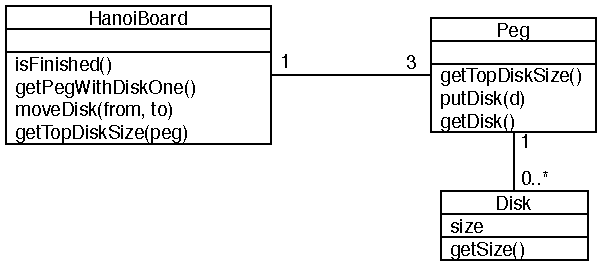
\includegraphics[scale=0.9]{img/hanoi-design.pdf}
\end{center}
\end{Slide} 

\begin{Slide}{Lösningsidé}
\begin{itemize}
 \item I \Emph{udda} drag; drag nr 1, 3, \ldots\  flyttar man den minsta brickan, bricka 1, till pinnen närmast till höger. Pinne 1 anses därvid finnas till höger om pinne 3.
 \item I \Emph{jämna} drag; drag nr 2, 4, \ldots\  flyttar man en bricka mellan de två pinnar som inte innehåller bricka 1.
\end{itemize}
\end{Slide} 


%
%\begin{frame}[fragile=singleslide]
%\frametitle{Scenario}
%\begin{itemize}
%\item Lägg brickorna på pinne 1.
%\item Så länge spelet inte är slut:
%\item om udda drag:
%\begin{itemize}
%	 \item tag reda på numret på pinnen där bricka 1 finns
%	 \item flytta den översta brickan från denna pinne till
%	  pinnen närmast till höger
%\end{itemize}
%\item annars (om jämnt drag):
%\begin{itemize}
%	 \item tag reda på numret på pinnen där bricka 1 finns
%	 \item räkna ut numren på de båda andra pinnarna
%	 \item flytta den minsta brickan mellan dessa pinnar
%\end{itemize}
%\end{itemize}
%\end{frame} 
%

%
%\begin{frame}[fragile=singleslide]
%\frametitle{\code{Disk}, en bricka}
%\FIXBEFORECODE
%\begin{Code}
%public class Disk {
%	private int size;
%	
%	/** Skapar en bricka med storleken size */
%	public Disk(int size) {
%		this.size = size;
%	}
%	
%	/** Tar reda på brickans storlek */
%	public int getSize() {
%		return size;
%	}
%}
%\end{Code}
%\end{frame} 
%
%\begin{frame}[fragile=singleslide]
%\frametitle{\code{Peg}, en pinne}
%\FIXBEFORECODE\FIXBEFORECODE
%\begin{Code}
%public class Peg {
%	private ArrayList<Disk> disks;
%	
%	public Peg() { disks = new ArrayList<Disk>(); }
%	
%	public int getTopDiskSize() {
%		return (! disks.isEmpty()) ?
%		       disks.get(disks.size() - 1).getSize() :
%		       Integer.MAX_VALUE;
%	}
%	
%	public void putDisk(Disk d) { 
%		disks.add(d); 
%	}
%	
%	public Disk getDisk() {
%		Disk d = disks.remove(disks.size() - 1);
%		return d;
%	}
%}
%\end{Code}
%\end{frame} 
%
%\begin{frame}[fragile=singleslide]
%\frametitle{\code{HanoiBoard}, spelplanen, 1}
%\FIXBEFORECODE\FIXBEFORECODE
%\begin{Code}
%public class HanoiBoard {
%	private Peg[] pegs;
%	
%	public HanoiBoard(int nbrDisks) {
%		pegs = new Peg[3];
%		for (int i = 0; i < pegs.length; i++) {
%			pegs[i] = new Peg();
%		}
%		for (int i = nbrDisks; i >= 1; i--) {
%			pegs[0].putDisk(new Disk(i));
%		}
%	}
%	
%	public int getPegWithDiskOne() {
%		int peg1 = 0;
%		while (getTopDiskSize(peg1) != 1) {
%			peg1++;
%		}
%		return peg1;
%	}
%\end{Code}
%\end{frame} 
%
%\begin{frame}[fragile=singleslide]
%\frametitle{\code{HanoiBoard}, spelplanen, 2}
%\FIXBEFORECODE
%\begin{Code}
%	public boolean isFinished() {
%		return isEmpty(0) &&
%		       (isEmpty(1) || isEmpty(2));
%	}
%	
%	public int getTopDiskSize(int peg) {
%		return pegs[peg].getTopDiskSize();
%	}
%	
%	public void moveDisk(int from, int to) {
%		Disk d = pegs[from].getDisk();
%		pegs[to].putDisk(d);
%	}
%	
%	private boolean isEmpty(int peg) {
%		return pegs[peg].getTopDiskSize() ==
%		       Integer.MAX_VALUE;
%	}
%}
%\end{Code}
%\end{frame} 
%
%\begin{frame}[fragile=singleslide]
%\frametitle{\code{HanoiStrategy}, algoritmen, 1}
%\FIXBEFORECODE
%\begin{Code}
%public class HanoiStrategy {
%	private HanoiBoard board;
%	
%	public HanoiStrategy(HanoiBoard board) {
%		this.board = board;
%	}
%	
%	public void moveDisks() {
%		int moveNbr = 1;
%		while (! board.isFinished()) {
%			moveOneDisk(moveNbr);
%			moveNbr++;
%		}
%	}
%\end{Code}
%\end{frame} 
%
%\begin{frame}[fragile=singleslide]
%\frametitle{\code{HanoiStrategy}, algoritmen, 2}
%\FIXBEFORECODE \FIXBEFORECODE
%\begin{Code}
%	private void moveOneDisk(int moveNbr) {
%		int peg1 = board.getPegWithDiskOne();
%		int from; // pinne att flytta en bricka från
%		int to;   // pinne att flytta en bricka till
%		if (moveNbr % 2 != 0) {
%			from = peg1;
%			to = (from + 1) % 3;
%		} else {
%			from = (peg1 + 1) % 3;
%			to = (from + 1) % 3;
%			if (board.getTopDiskSize(from) > 
%			    board.getTopDiskSize(to)) {
%				int temp = from;
%				from = to;
%				to = temp;
%			}
%		}
%		System.out.println(...);
%		board.moveDisk(from, to);
%	}
%\end{Code}
%\end{frame} 
%
%\begin{frame}[fragile=singleslide]
%\frametitle{\code{TowersOfHanoi}, \code{main}-metoden}
%\begin{Code}
%import java.util.Scanner;
%
%public class TowersOfHanoi {
%	public static void main(String[] args) {
%		System.out.print("Antal brickor: ");
%		Scanner scan = new Scanner(System.in);
%		int nbrDisks = scan.nextInt();
%		HanoiBoard board = new HanoiBoard(nbrDisks);
%		HanoiStrategy strategy = new HanoiStrategy(board);
%		strategy.moveDisks();
%	}
%}
%\end{Code}
%\end{frame} 

\Subsection{Inbjuden gäst: Patrik Persson lajvkodar androidapp}
\begin{Slide}{Designexempel: Skriv en app för Andorid}
\begin{itemize}
\item Med de kunskaper ni tillgodogör er i denna kurs är det hyffsat lätt att komma i gång med utveckling av mobilappar i den integrerade utvecklingsmiljön \href{https://en.wikipedia.org/wiki/Android_Studio}{Android Studio}.
\item Läs mer \href{http://techworld.idg.se/2.2524/1.602344/premiar-for-android-studio}{på techworld} och \href{http://developer.android.com/develop/index.html}{på officiella hemsidan}.
\item Inbjuden gästföreläsare Patrik Persson lajvkodar androidapp i Android Studio...
\end{itemize}
\begin{center}

\includegraphics[width=0.6\textwidth]{img/android-studio}
\end{center}
\end{Slide}


\begin{Slide}{Grumligtlådan}
\begin{tabular}{r|l}
\#Lappar  & Ämne                         \\ \hline
6  & \Emph{StringBuilder}\\
3  & \Emph{Vektorer, ArrayList}\\
2  & \Emph{Implementering och användning av klasser}\\
2  & \Emph{Sorteringsalgoritmer}\\
2  & Static\\
1 & Arv\\
1  & Generics\\
1  & for-each-sats\\
1  & Flera metoder med samma namn\\
1  & Matris\\
1  & När du säger "Java" exakt vad menar du då?\\
1  & Iterator\\
1 & Volatile Image\\
\end{tabular}
\end{Slide}

\begin{Slide}{Övning: Dictionary}\footnotesize
Implementera denna klass som har hand om en ordlista. \\Använd en vektor \code{String[] words} för att spara orden.
\begin{ClassSpec}{Dictionary}
/** Skapar en ny ordlista */
Dictionary();

/** Sätt in ett nytt ord på rätt plats i listan */
void insertWord(String w);

/** Returnerar listans ord som, skilda med mellanslag */
String toString();

/** Returnerar true om ordet finns i listan, annars false */
boolean contains(String word);
\end{ClassSpec}
\vspace{1em}
Extraövning: Byt attributrepresentationen till \code{ArrayList<String>}
\end{Slide}

\end{document}